\documentclass[12pt]{article}
\usepackage{amssymb, amsthm, amsmath, amsfonts}
\usepackage{fancybox, multicol}
\usepackage{graphicx}
\usepackage{amsrefs}
\usepackage{type1cm, color, array}
\usepackage{bardtex}
\usepackage{verbatim}

\styleoption{poster}

\usepackage{fourier}

%The following three optional commands change the colors in the poster; if you want to change the default colors, use any or all of these three commands by removing the % symbols, and inserting your choice of colors.  See the manual for details about colors in posters.
\definecolor{BardRed}{cmyk}{0.00,1.00,0.75,0.30}
\definecolor{EHBlack}{cmyk}{0.00,0.00,0.00,0.85}

\boxcolor{EHBlack}
\toptitlecolor{BardRed}
\boxtitlecolor{EHBlack}

%The following three optional commands insert figures to the left and/or right of the title box; if you want to insert such figures, use either the first command (for the same figure on both sides of the title box), or one or both of the second and third commands (for a figure on only one side of the title box, or for different figures on the two sides).  See the manual for details these commands.
%\leftrightlogo{math_prog_logo.pdf}
\leftlogo{eh_logo.png}
\rightlogo{cs_logo.pdf}

%The following optional command allows the replacement of the word ``adviser'' in the poster top with one of ``advisers,'' ``advisor'' or ``advisors."  If the command is not used, the default is ``adviser.''
%\adviseroption{adviser}

%The following optional command allows the replacement of the word ``program'' in the program top with ``programs."  If the command is not used, the default is ``program.''
%\programoption{program}

%The following optional command allows for a change in the style of the poster.  The options are ``styleone,'' ``styletwo,'' ``stylethree'' or ``stylefour."  If the command is not used, the default is ``styleone.''
\posterstyle{stylefour}

%Your macros, if you have any.

\begin{document}

\begin{posterbard}

%\postertop {Senior Project Posters in LaTeX }{Helga Homology}{Mathematics}{May 2099}{Calvin Calculus}

%scale values 1 -> 2 without logo
%scale values 1 -> 1.6 with math_prog_logo.pdf logos, or other logos that have roughly the same height and width
\postertopscale {Don't Take This Personally: Sentiment Analysis for Identification of \textit{``Subtweeting''} on Twitter}{Noah Segal-Gould}{Experimental Humanities Concentration and Computer Science}{May 2018}{Sven Anderson}{1.4}

\begin{posterboxtitle}{Introduction} 
Twitter is a news and social networking service to which users send text posts called \textbf{tweets}. The OED defines \textcolor{WildStrawberry}{``subtweet''} as a \textbf{tweet} ``...that refers to a particular user without directly mentioning them, typically as a form of furtive mockery or criticism.''
\begin{center}
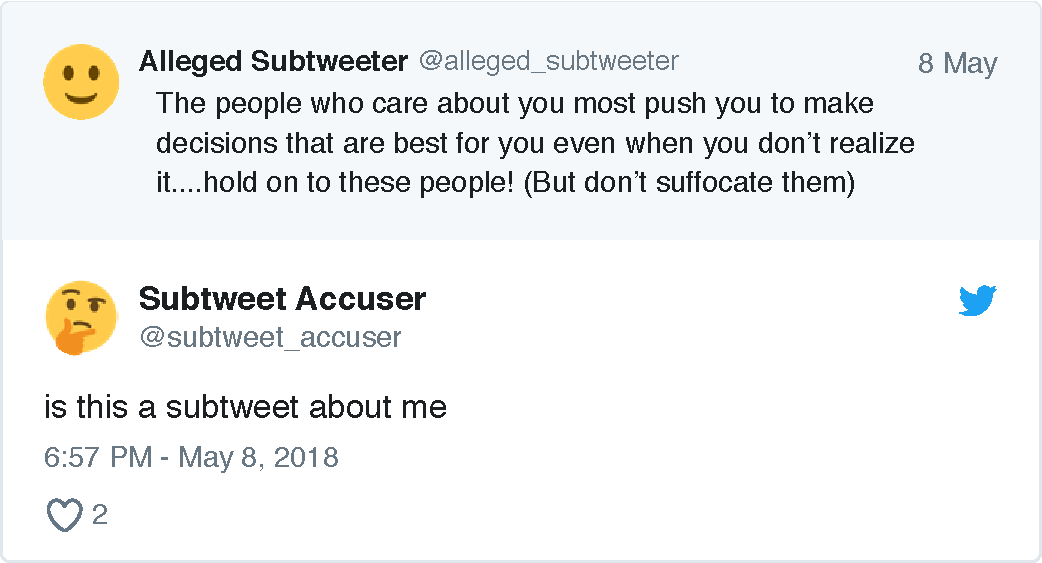
\includegraphics[width=\textwidth]{subtweet_example_1.pdf}\\
Figure 1: A Subtweet and a Reply Which Acts as an Accusation
\end{center}

\begin{itemize}
\item This project monitors the content of \textbf{replies} to acquire a dataset of \textcolor{WildStrawberry}{known subtweets} and \textcolor{Cyan}{known non-subtweets} because one does not already exist.
\item Tweets are classified as either \textcolor{WildStrawberry}{predicted subtweets} or \textcolor{Cyan}{predicted non-subtweets}.
\item An automated program which accesses Twitter (a Twitter bot) interacts with \textcolor{WildStrawberry}{subtweets} in real time.
\end{itemize}

\end{posterboxtitle}


\begin{posterboxtitle}{The Ground Truth Dataset}
This project treats identification of \textcolor{WildStrawberry}{subtweets} as a text classification problem. Supervised machine learning on text through classification typically requires some \textbf{ground truth dataset} of how specific documents ought to be categorized prior to any actual machine learning.

\begin{itemize}
\item For this project, \textcolor{WildStrawberry}{known subtweets} and \textcolor{Cyan}{known non-subtweets} were acquired using the Twitter search API with a query which exclusively selects tweets with \textbf{replies} which themselves \textit{contain} or \textit{exclude} the string \textbf{``subtweet''}.
\item This generalization was developed with \textbf{call-out culture} in mind. A particular pattern was observed that Twitter users often call-out subtweets from their peers in order to ask if they are the target or complain about the very act of subtweeting.
\item This method for data acquisition was a \textit{fast and cheap} way to gather data for training the classifier, but a tweet is not necessarily a \textcolor{WildStrawberry}{subtweet} just because a user \textit{happens} to reply to it with or without the string \textbf{``subtweet''}.
\end{itemize}

Whereas the ground truth dataset acquisition process necessarily relies on \textbf{replies}, the actual classification \textbf{deliberately excludes them} in favor of pure text classification in order to classify tweets live without the need for any users to have already interacted with them. \textbf{Figure~1} shows a tweet which is present in the ground truth dataset and a reply which was used to identify it as a \textcolor{WildStrawberry}{subtweet}.

\end{posterboxtitle}


\begin{posterboxtitle}{Training \& Testing the Classifier}
\begin{itemize}
\item The \textbf{Naive Bayes} classification algorithm makes use of \textbf{Bayes Rule} to predict the likelihood that a particular set of features (e.g. words) belong to a particular class~\cite{naive_bayes}.
\item It makes the \textbf{naive} assumption that the features are conditionally independent: the \textit{presence} or \textit{omission} of a particular feature does not change the likelihood of encountering other features within that class.
\end{itemize}
\[{\text{Pr}(\text{class}|\text{word})}=\frac{\text{Pr}(\text{word}|\text{class})\text{Pr}(\text{class})}{P(\text{word})}\] 
\noindent
\textbf{Naive Bayes} computes the product of all the predicted probabilities for each word in the document. The greatest product computed across all the classes becomes the predicted class for that document.

\begin{itemize}
\item $k$-folds cross-validation was used to split apart \textbf{training} and \textbf{testing} sections of the ground truth dataset~\cite{k_folds}. 
\item For each fold $k_{i}$, the algorithm selects different sections of the entire dataset as the \textbf{training} and \textbf{testing} sets within that fold.
\item The statistics on the performance of the classifier are computed for that fold alone and averaged across all folds to measure the overall performance of the classifier.
\end{itemize}
\begin{center}
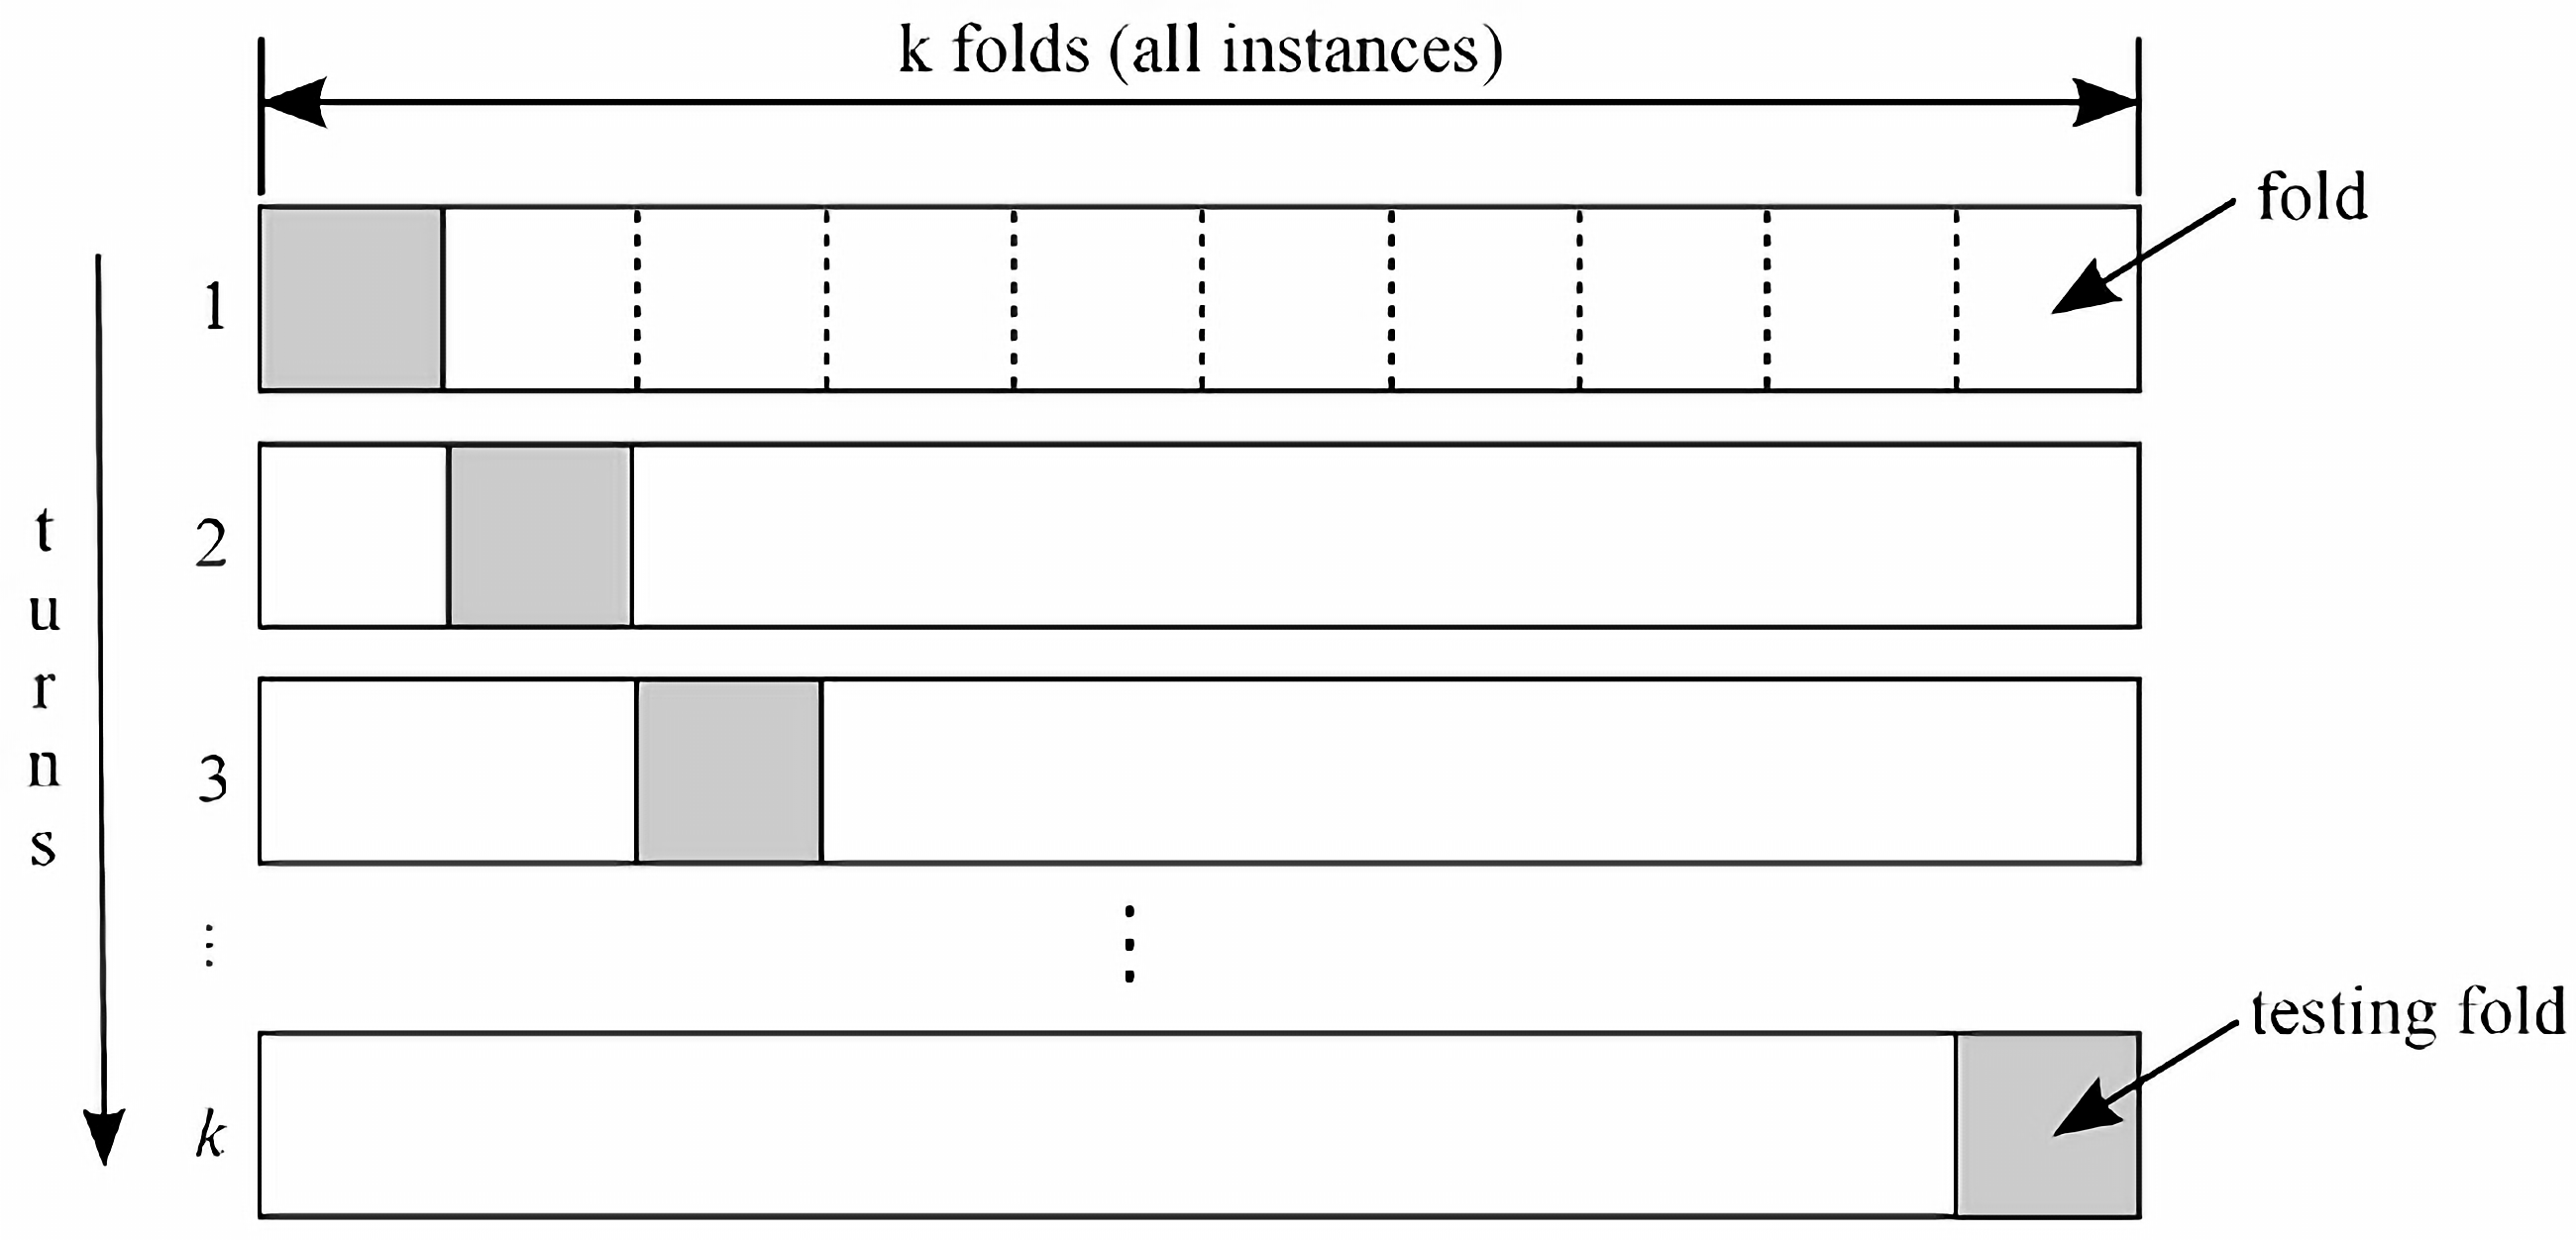
\includegraphics[width=\textwidth]{k_folds_new.png}\\
Figure 2: $k$-folds Cross-Validation Example \cite{k_folds}
\end{center}

To measure the performance of the classifier, it is necessary to keep track of how many \textbf{correct} and \textbf{incorrect} predictions it makes. These predictions are quantified in terms of \textbf{true positives}, \textbf{true negatives}, \textbf{false positives}, and \textbf{false negatives}.
\begin{itemize}
\item \textbf{True positives} (TP) are \textcolor{WildStrawberry}{known subtweets} which were \textbf{correctly} classified as \textcolor{WildStrawberry}{predicted subtweets}.
\item \textbf{True negatives} (TN) are \textcolor{Cyan}{known non-subtweets} which were \textbf{correctly} classified as \textcolor{Cyan}{predicted non-subtweets}.
\item \textbf{False positives} (FP) are \textcolor{Cyan}{known non-subtweets} which were \textbf{incorrectly} classified as \textcolor{WildStrawberry}{predicted subtweets}.
\item \textbf{False negatives} (FN) are \textcolor{WildStrawberry}{known subtweets} which were \textbf{incorrectly} classified as \textcolor{Cyan}{predicted non-subtweets}.
\end{itemize}
Thus, the performance of the classifier is measured in terms of precision, recall, and F1 score.
\begin{alignat*}{2}
  \text{Precision}=\frac{TP}{TP+FP}  &\qquad \text{Recall}=\frac{TP}{TP+FN} 
\end{alignat*}

\[F_{1}=\frac{2*(\text{Precision}*\text{Recall})}{\text{Precision}+\text{Recall}}\]

\begin{center}
	\begin{tabular}{ | p{8em} | p{5em} | p{5em} | p{5em} | }
		\hline
		&Precision&Recall&$F_{1}$ Score
		\\ 
		\hline
		\textcolor{cyan}{non-subtweets}&0.7357&0.6988&0.7166
		\\ 
		\hline
		\textcolor{WildStrawberry}{subtweets}&0.7132&0.7490&0.7305
		\\
		\hline
	\end{tabular}
	\medskip
	\\Table 1: Statistics Averaged Across 10 Folds of Cross-Validation
\end{center}

\end{posterboxtitle}

\begin{posterboxtitle}{Confusion Matrix}
\noindent
\textbf{Figure~3} is a confusion matrix which illustrates this performance in terms of raw counts and normalized over the entire ground truth dataset.
\begin{center}
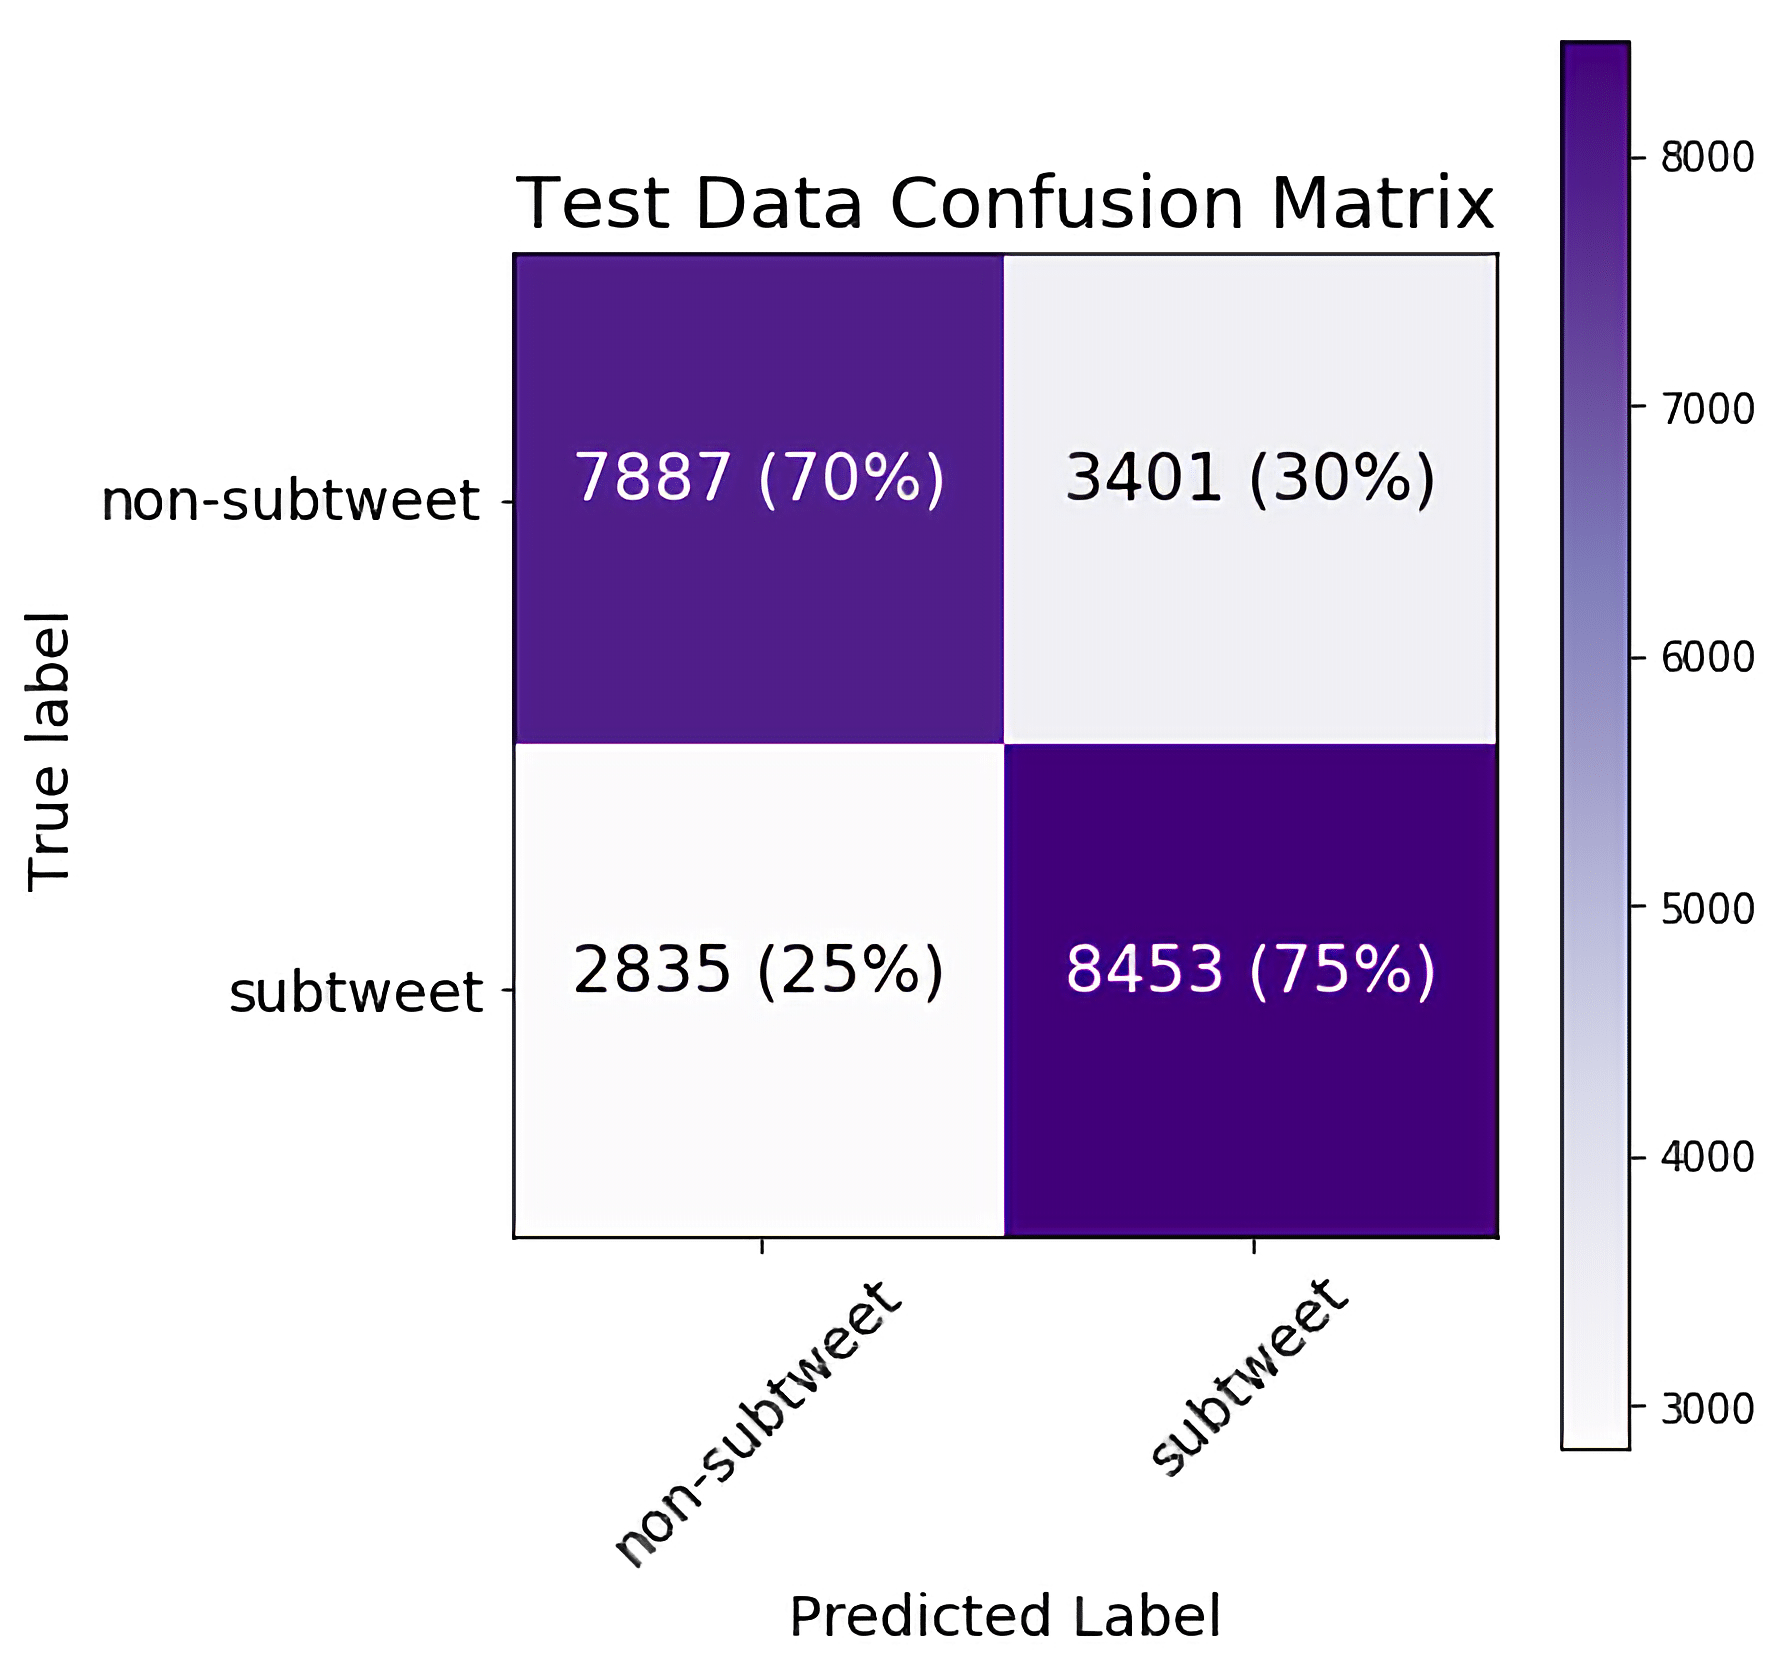
\includegraphics[width=\textwidth]{confusion_matrix_new.png}\\
Figure 3: Accumulated Confusion Matrix for All 10 Folds
\end{center}

\end{posterboxtitle}

\begin{posterboxtitle}{The Twitter Bot}
After training and testing the classifier, it was utilized to create a Twitter bot which interacts with \textcolor{WildStrawberry}{predicted subtweets} in real time. It announces subtweets as they are posted in order to present covertly hurtful content as obviously hurtful in a public fashion. \textbf{Figure~4} shows a (censored) example of the bot quoting a user's tweet.
\begin{center}
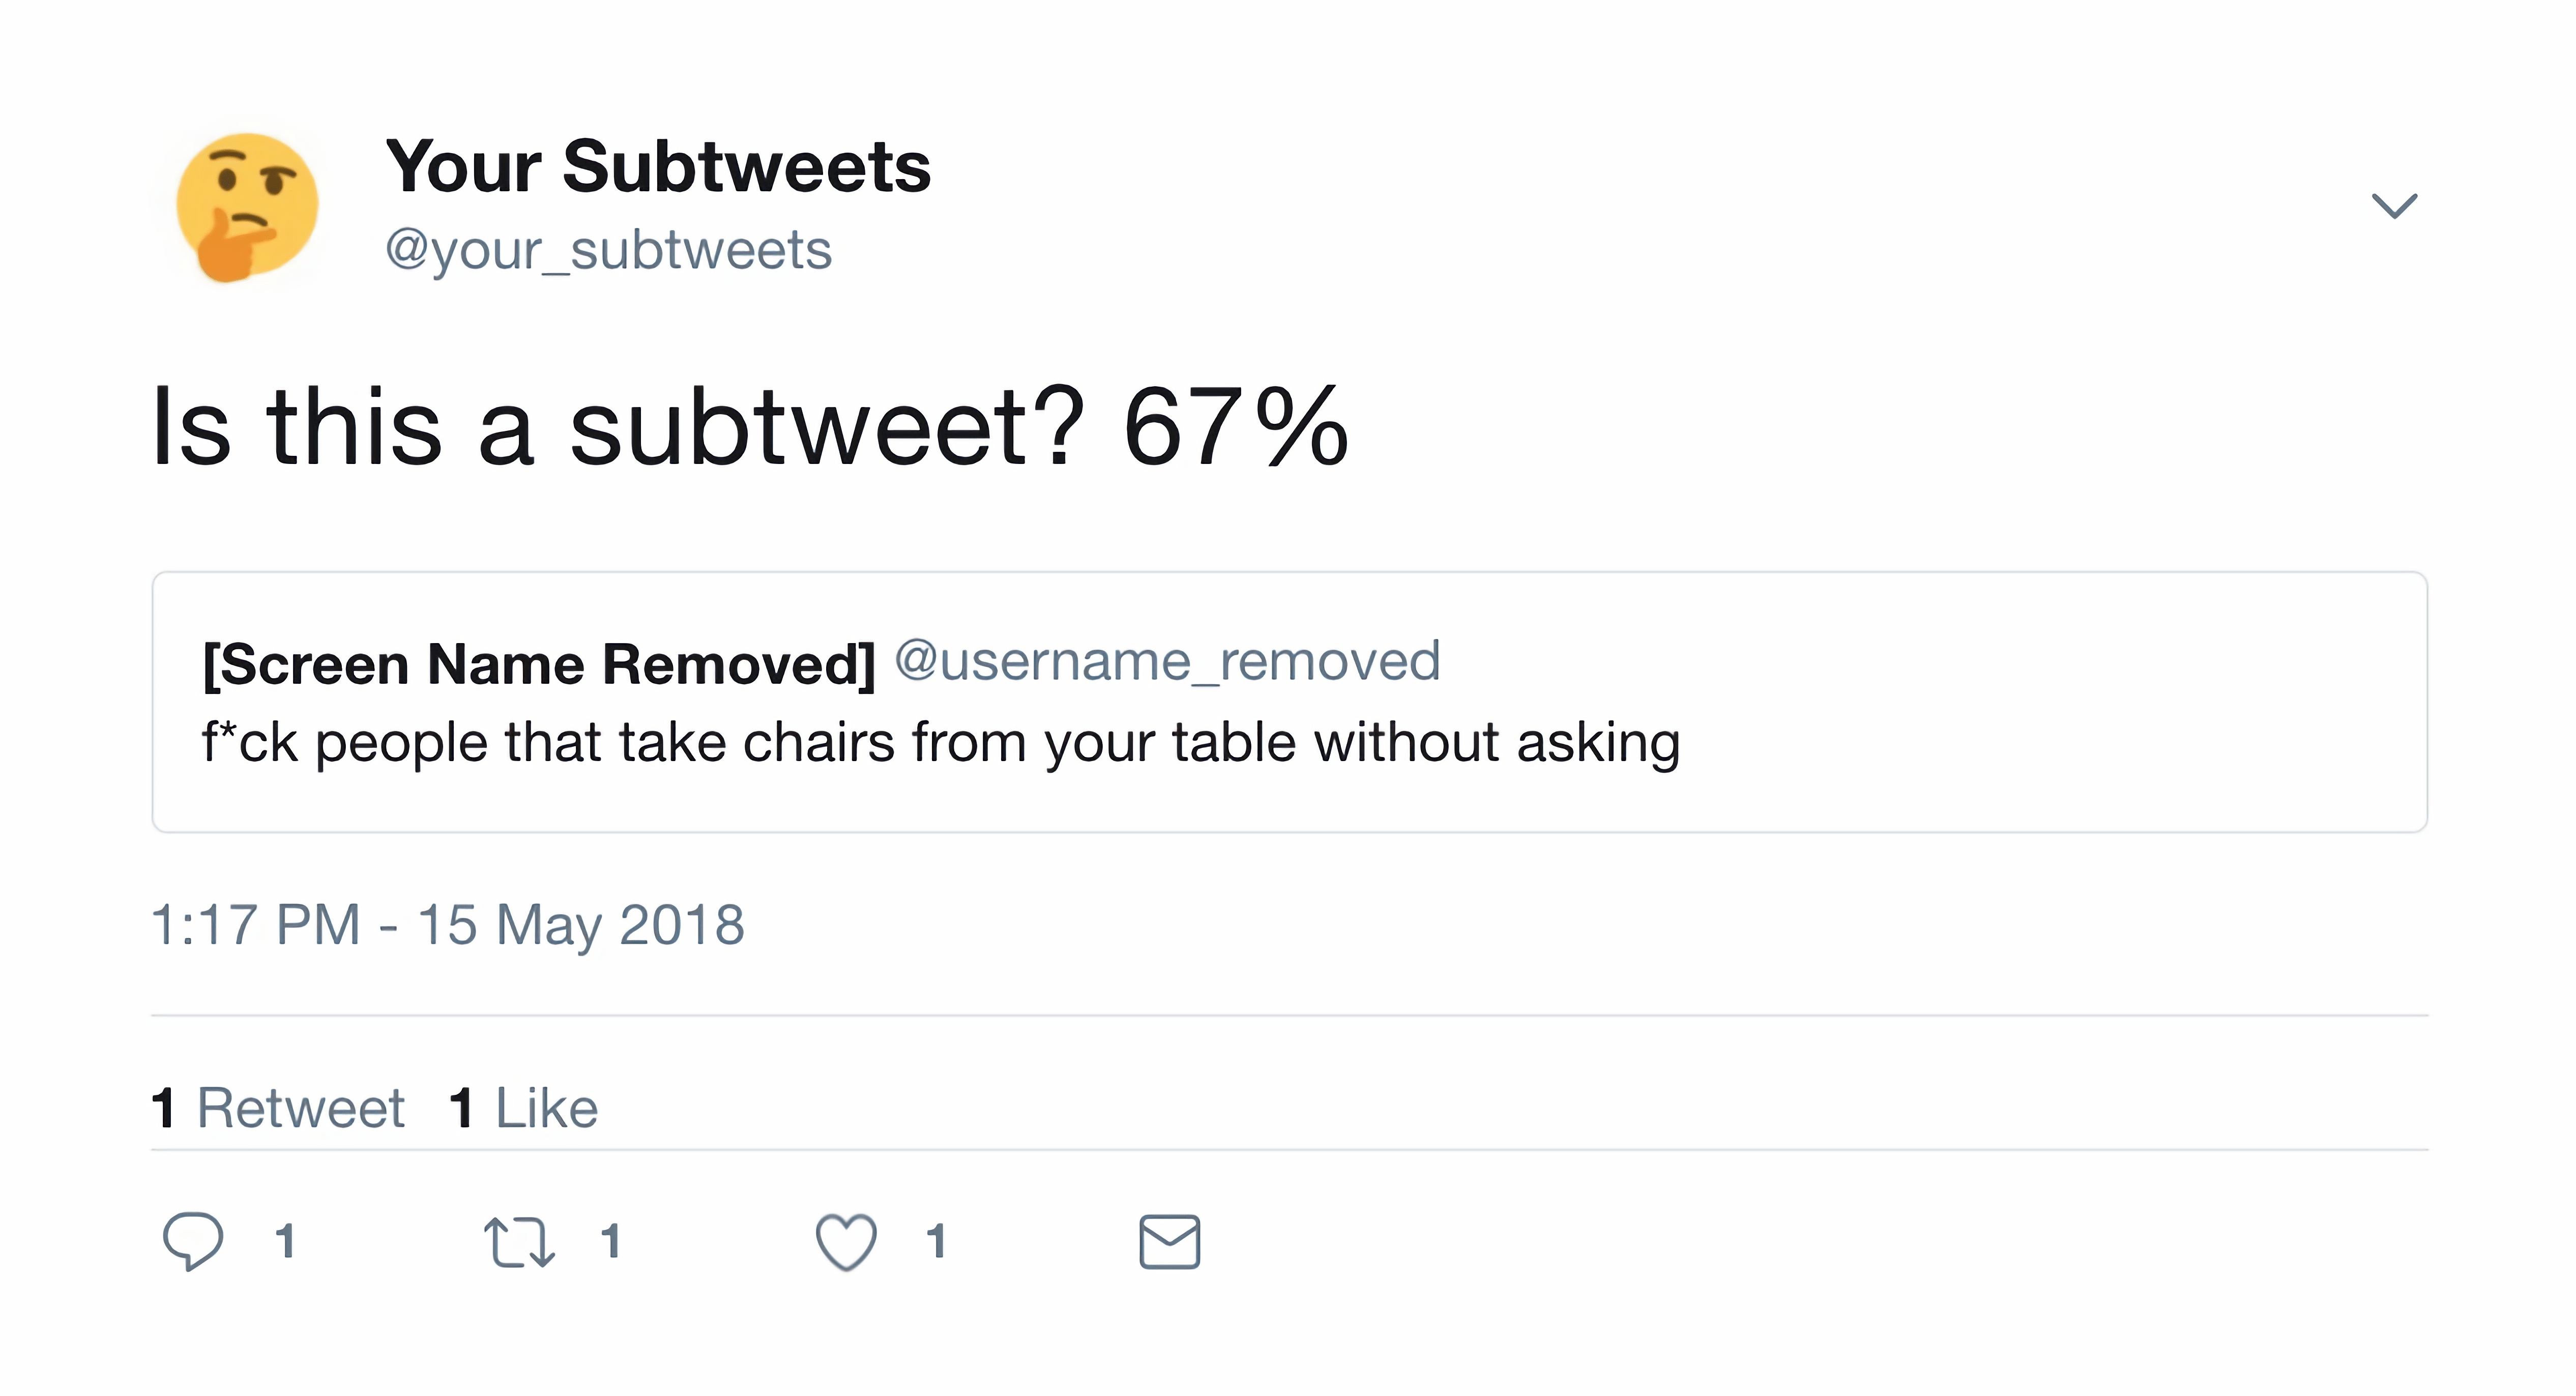
\includegraphics[width=\textwidth]{quote_example_new.png}\\
Figure 4: Example of the Twitter Bot Quoting a Tweet
\end{center}
\end{posterboxtitle}

\begin{bibliog}

\bib{naive_bayes}{article}{
	title={The optimality of naive Bayes},
	author={Zhang, Harry},
	journal={AA},
	volume={1},
	number={2},
	pages={3},
	date={2004}
}

\bib{k_folds}{article}{
	author={Borovicka, Tomas},
	author={Jirina Jr, Marcel},
	author={Kordik, Pavel},
	author={Jirina, Marcel},
	title={Selecting representative data sets},
	date={2012}
}

\end{bibliog}


\end{posterbard}

\end{document}

%%%%%%%


\newcommand{\postertoptwo}[5]{
\begin{center} 
\begin{tabular}{ m{0.13\textwidth}  m{0.66\textwidth}  m{0.13\textwidth} }
%\vfill 
\begin{center}
\leftlogofig
\end{center}
%\vfill 
 &
\begin{center}
\begin{Sbox}
\begin{minipage}{0.55\textwidth}
\begin{center}
\textcolor{White}{\bf \fontsize{\titlefontsize}{\titlefontsize}\selectfont
 #1\\ \bigskip
\fontsize{\namefontsize}{\namefontsize}\selectfont
 #2 \qquad \fontsize{\advfontsize}{\advfontsize}\selectfont Adviser: #5\\ \bigskip\bigskip
\fontsize{\progdatefontsize}{\progdatefontsize}\selectfont 
#3 \pprogram, Bard College, #4}
\end{center}
\end{minipage}
\end{Sbox}
\setlength{\fboxrule}{0pt}%%%%%%%%
\setlength{\fboxsep}{20pt}
\fcolorbox{\boxxcolor}{\topptitlecolor}{\TheSbox}
 \end{center}
& 
%\vfill 
\begin{center}
\rightlogofig
\end{center}
%\vfill 
\\
\end{tabular}
\end{center}
\bigskip\bigskip
\fontsize{\boxfontsize}{1.2\boxfontsize} \selectfont
\setlength{\columnseprule}{0pt}
\setlength{\columnsep}{0.01\textwidth}
\setcounter{finalcolumnbadness}{0}
\begin{multicols}{3}\raggedcolumns
}


\newcommand{\postertopthree}[5]{
\begin{center} 
\begin{tabular}{ m{0.13\textwidth}  m{0.66\textwidth}  m{0.13\textwidth} }
%\vfill 
\begin{center}
\leftlogofig
\end{center}
%\vfill 
 &
%
%\begin{center}
%\begin{Sbox}
%\begin{minipage}{0.55\textwidth}
%\begin{center}
%\textcolor{White}{\bf \fontsize{\titlefontsize}{\titlefontsize}\selectfont
% #1\\ \bigskip
%\fontsize{\namefontsize}{\namefontsize}\selectfont
%#2 \qquad \fontsize{\advfontsize}{\advfontsize}\selectfont \addviser: #5\\ \bigskip\bigskip
%\fontsize{\progdatefontsize}{\progdatefontsize}\selectfont 
%#3 \pprogram, Bard College, #4}
%\end{center}
%\end{minipage}
%\end{Sbox}
%\setlength{\fboxrule}{0pt}%%%%%%%%
%\setlength{\fboxsep}{20pt}
%\fcolorbox{\boxxcolor}{\topptitlecolor}{\TheSbox}
% \end{center}
%
              \begin{center}
                  \begin{Sbox}
                    \begin{minipage}{0.55\textwidth}
                      \parindent=-20pt
                      \setlength{\fboxsep}{25pt}
                       \fcolorbox{\topptitlecolor}{\topptitlecolor}
                       {
                       \begin{minipage}{\textwidth}
                        \fontsize{\boxheadingfontsize}{1.2\boxheadingfontsize} \selectfont
                        \begin{center}
                          \textcolor{White}{\bf \fontsize{\titlefontsize}{\titlefontsize}\selectfont #1}
                      \end{center}
                      \end{minipage}
                      }\par
                      \parindent=20pt
                      $\ $\par 
                      \bigskip      
                      \begin{center}
                      \fontsize{\namefontsize}{\namefontsize}\selectfont
 #2 \qquad \fontsize{\advfontsize}{\advfontsize}\selectfont \addviser: #5\\ \bigskip\bigskip
\fontsize{\progdatefontsize}{\progdatefontsize}\selectfont 
#3 \pprogram, Bard College, #4
\end{center}
              \end{minipage}
                  \end{Sbox}
                  \setlength{\fboxrule}{0pt}%%%%%%%%
                  \setlength{\fboxsep}{0pt}
                  \fcolorbox{\boxxcolor}{White}{\TheSbox}
                \end{center}\bigskip\bigskip\bigskip
& 
%\vfill 
\begin{center}
\rightlogofig
\end{center}
%\vfill 
\\
\end{tabular}
\end{center}
\bigskip\bigskip
\fontsize{\boxfontsize}{1.2\boxfontsize} \selectfont
\setlength{\columnseprule}{0pt}
\setlength{\columnsep}{0.01\textwidth}
\setcounter{finalcolumnbadness}{0}
\begin{multicols}{3}\raggedcolumns
}




